\section{Term-Template: Rewriting Metafunction Applications}

Since metafunction applications have the following shape - `(metafunction-name term-template ...)` these can be detected quite trivially given a list of defined metafunctions. 

\subsection{Algorithm}
Term-template is visited recursively. Let $Mf$ be the set of metafunction names. When visiting $t_{in}=\text{\TermSequence}$, check if $t_1$ is \TermLiteral where $l=\text{Variable}$ and $v \in Mf$. Return \ApplyMetafunction with $n=v$ and $t=t_{in}$.

$t_{in}$ contains InArg and MatchRead annotations. These are handled in the following way:

\begin{itemize}
\item
InArg annotations are left intact. Signatures of both `TermSequence` and `ApplyMetafunctions` must match.
\item
MatchRead annotations can be safely removed. None of such variable assignments are used to generate $t_{in}$.
\end{itemize}

\subsection{Example}

The example shown in Figure \ref{transformation-term-mfapply} displays transformation described above given a set of meta-function names only containing single \texttt{set-contains?}. Since the first element of \texttt{TermSequence} is \texttt{Variable} term-template with suitable name, additional \texttt{MetafunctionApplication} term is added.

\begin{figure}[H]
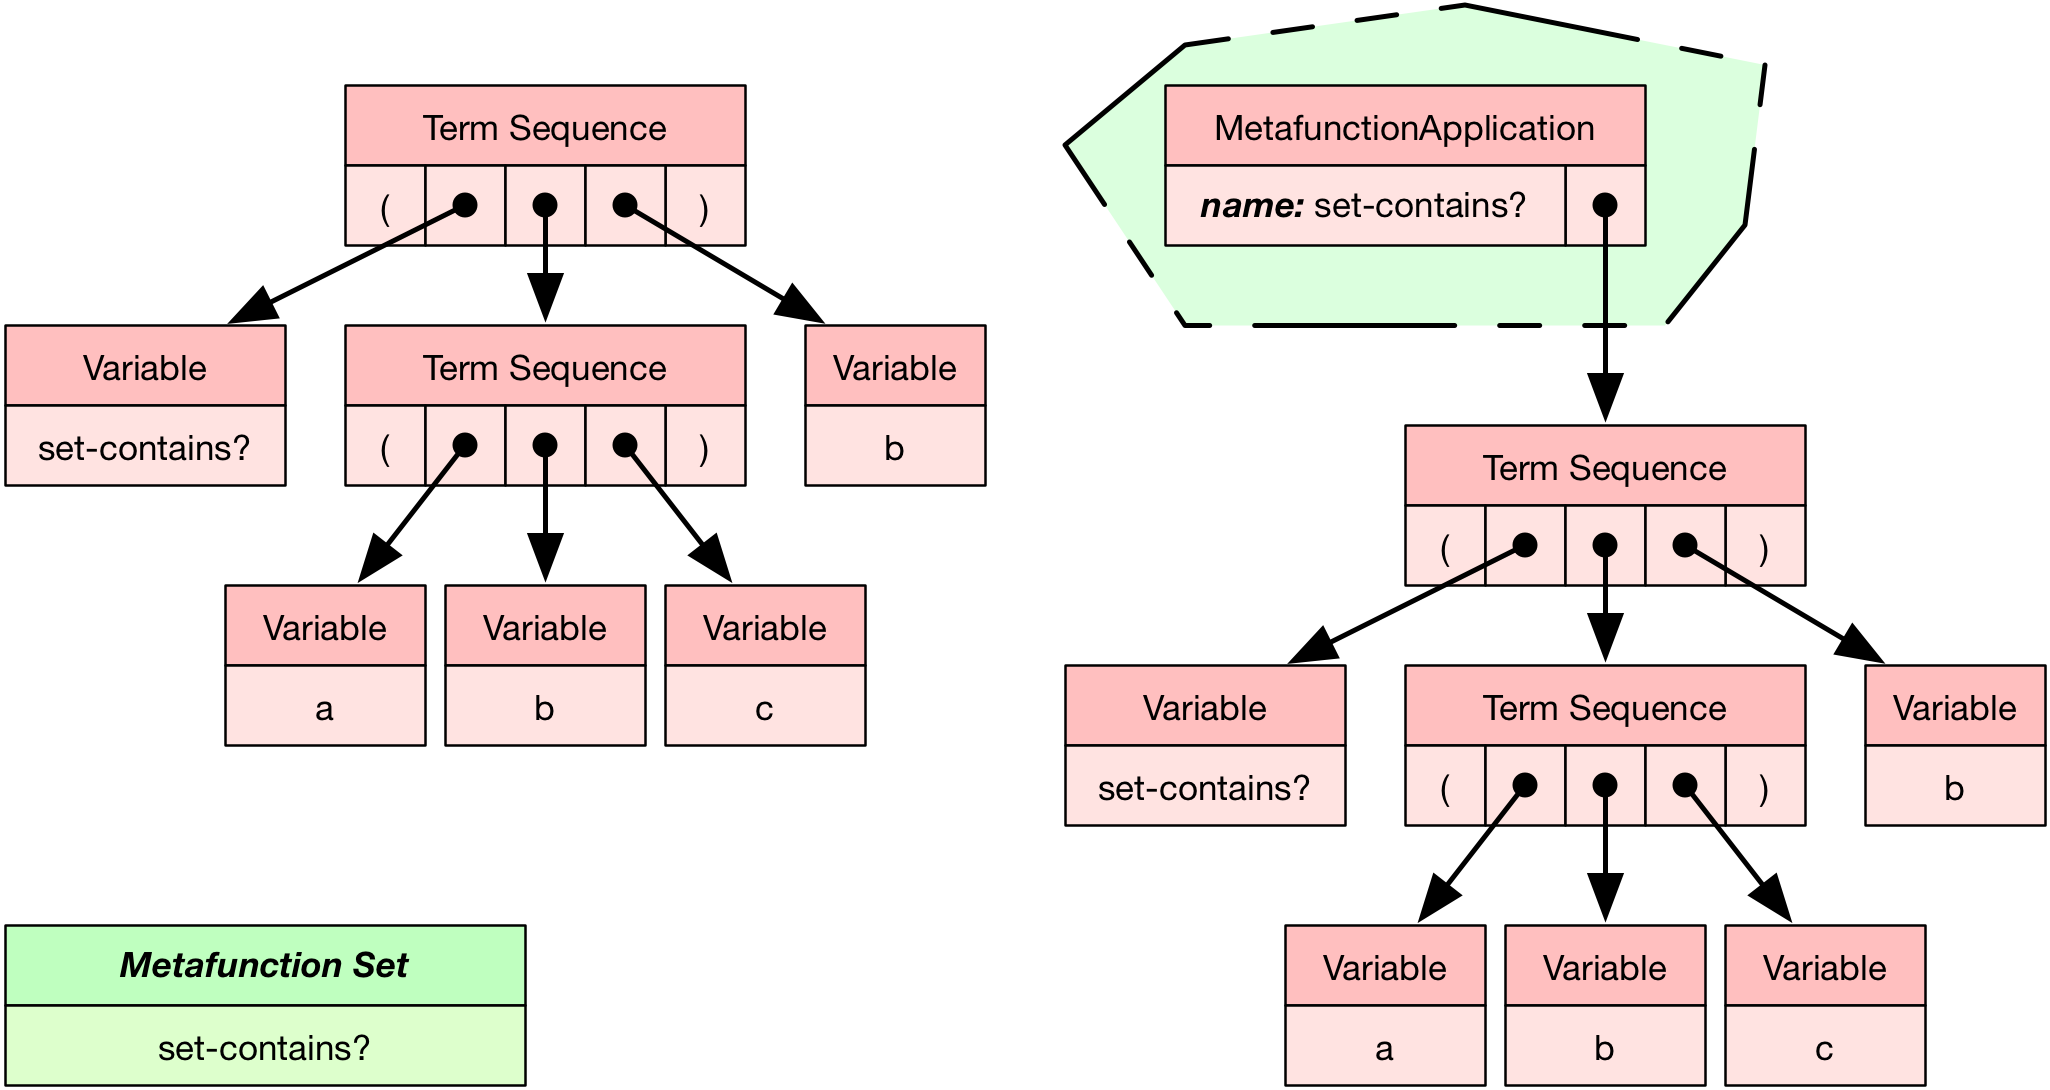
\includegraphics[scale=0.20]{transformation-term-mfapply.png}
\caption{Term-template before and after applying metafunctions.}
\label{transformation-term-mfapply}
\end{figure}
